% !TEX encoding = UTF-8 Unicode
\documentclass[10pt]{beamer}

\usepackage{polyglossia}
\usepackage{fontspec}
\usepackage{csquotes}
\usepackage{microtype}
\usepackage{tikz}
\usepackage{color}
\usepackage[backend=biber,style=iso-authoryear,sortlocale=cs_CZ,autolang=other,bibencoding=UTF8]{biblatex}
\usepackage{booktabs}
\usepackage{hyperref}

\usetikzlibrary{decorations.pathreplacing}
\usetikzlibrary{calc}
\setmainlanguage{czech}
\setmainfont{TeX Gyre Termes}
\usetheme{Boadilla}
\usecolortheme{crane}
\setbeamertemplate{section in toc}[ball unnumbered]
\addbibresource{zotero.bib}

\hypersetup{
	pdfencoding=auto,
	unicode=true,
	citecolor=green,
	filecolor=blue,
	linkcolor=red,
	urlcolor=blue
}

\makeatletter
\newcommand*{\currentSection}{\@currentlabelname}
\makeatother

\newcommand{\mat}{\mathbb}

\title[Hierarchické modely síťového provozu]
{
	Hierarchické modely síťového provozu
}

\titlegraphic
{
	
\includegraphics[width=0.2\columnwidth]{images/fjfi.png}
}

\author[Marek Dědič]
{
	Marek~Dědič\inst{1} \\
	Školitel:~Ing.~Tomáš~Pevný,~Ph.D.\inst{2}
}

\institute[FJFI ČVUT v Praze]
{
	\inst{1} ČVUT v Praze, Fakulta jaderná a fyzikálně inženýrská, Matematická informatika \and
	\inst{2} Cisco Systems Inc., Karlovo náměstí 10, Praha 2
}

\AtBeginSection[]{
	\begin{frame}{\currentSection}
		\tableofcontents[currentsection]
	\end{frame}
}

\begin{document}

\begin{frame}
	\titlepage
\end{frame}

\begin{frame}{Obsah}
	\tableofcontents
\end{frame}

\section{Motivace}
\begin{frame}{Motivace}
	\centering
	\textit{\enquote{100 percent of companies are calling malicious malware hosts}}

	\cite{_cisco_2014}
\end{frame}

\begin{frame}{Data}
	\centering
	\begin{tabular}{lrr}
		\toprule
		\null & \multicolumn{2}{c}{Počet adres} \\
		\cmidrule(l){2-3}
		Datový soubor & Legitimní & Malware \\
		\midrule
		Trénovací legitimní & 417 208 484 & 0 \\
		Trénovací směs & 17 390 889 & 34 359 733 \\
		Testovací legitimní & 1 522 255 052 & 0 \\
		Testovací směs & 2 855 992 & 4 051 944 \\
		\bottomrule
	\end{tabular}
\end{frame}

\section{Řešená úloha}
\begin{frame}{Adresa URL}
	\centering
	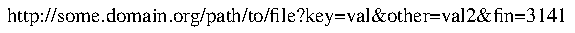
\includegraphics{images/url/url.pdf}
\end{frame}

\begin{frame}{Části adresy URL}
	\centering
	
\includegraphics{images/url_parts/url_parts.pdf}
\end{frame}

\begin{frame}{Části a tokeny adresy URL}
	\centering
	
\includegraphics{images/url_subparts/url_subparts.pdf}
\end{frame}

\section{MIL problém}
\begin{frame}{MIL problém}
	\centering
	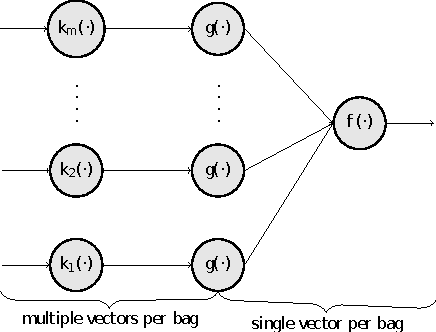
\includegraphics[width=0.7\columnwidth]{images/MIL.pdf}

	\cite{pevny_using_2016}
\end{frame}

\begin{frame}[label=doubleMIL]{Dvojitý MIL problém}
	\centering
	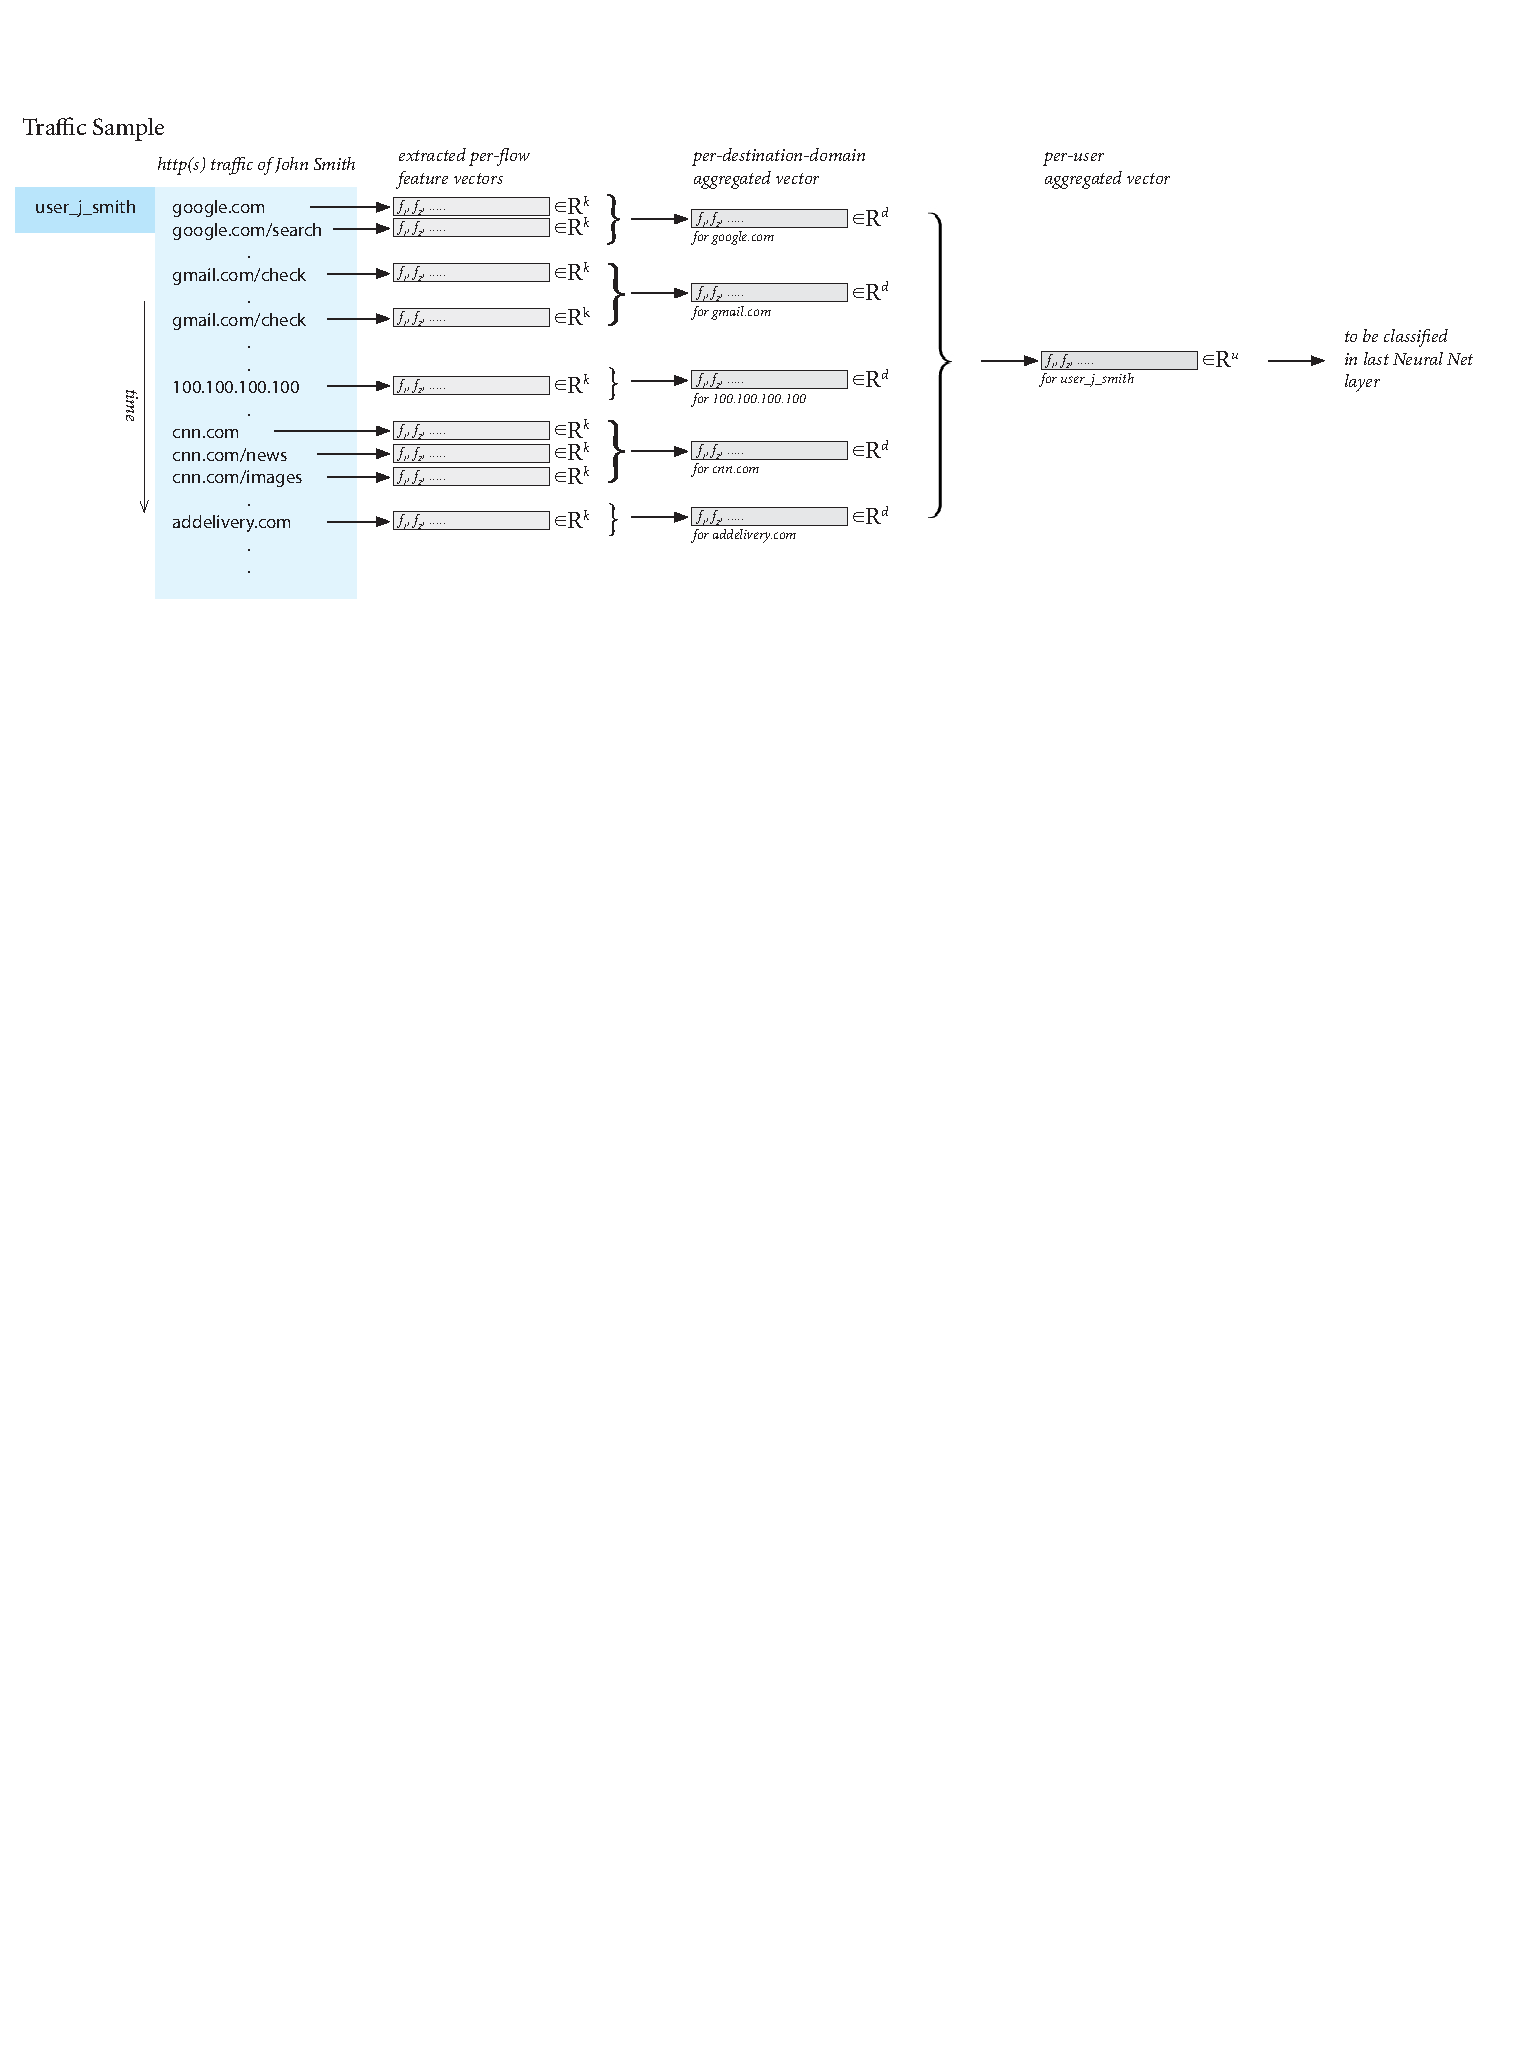
\includegraphics[width=0.9\columnwidth]{images/traffic.pdf}

	\cite{pevny_discriminative_2016}
\end{frame}

\section{Můj přínos}

\begin{frame}{Můj přínos}
	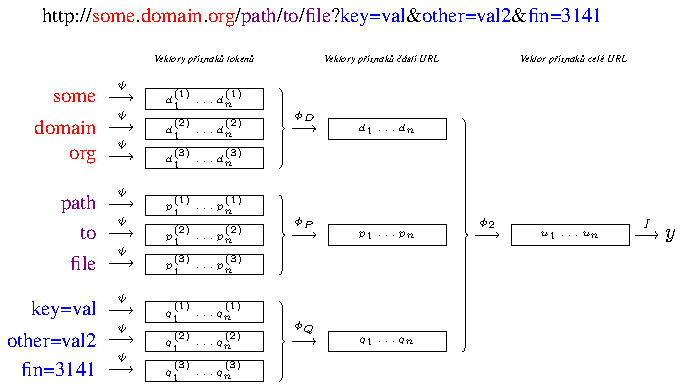
\includegraphics{images/model_modified_MIL/model_modified_MIL.pdf}

	\centering
\end{frame}

\section{Výsledky mé práce}
\begin{frame}{Výsledky mé práce}
	\centering
	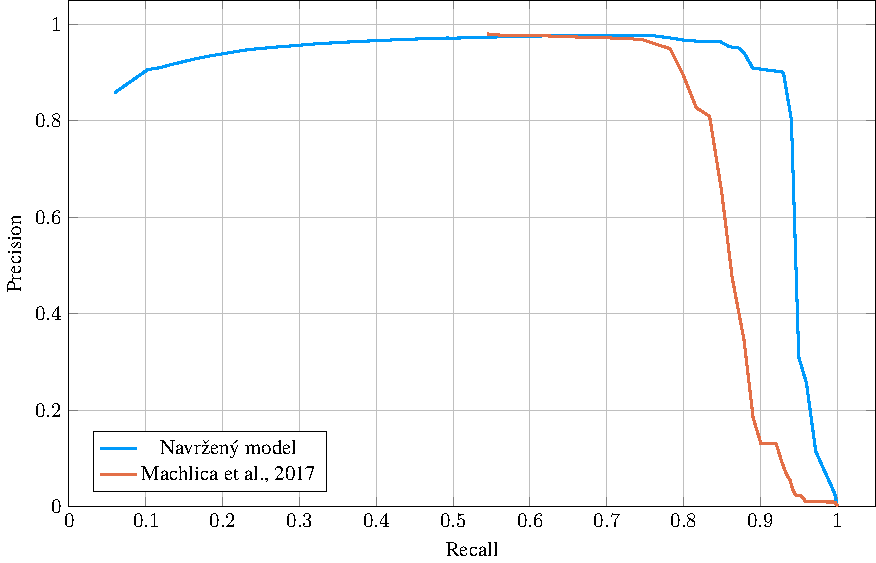
\includegraphics[width=0.9\columnwidth]{images/prior_art/prior_art.pdf}

	Srovnání s \cite{machlica_learning_2017}
\end{frame}

\begin{frame}{Seznam literatury}
	\printbibliography
\end{frame}

\begin{frame}[c]\frametitle{Blending feature extraction and classification}
	\vfill
	\begin{center}
		\begin{tikzpicture}
			\node (apple) at (0,0) {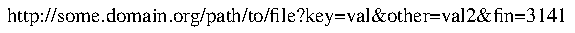
\includegraphics[trim = 30 30 30 30,width=1cm]{images/url/url.pdf}};
			\node (feature) at (4,0) {$x=(x_1,\ldots,x_d)$};
			\node (classifier) at (9,0) {$f(x)=\begin{cases} +1 \\ -1\end{cases}$};
				\draw [->] (apple.east) -- (feature.west) node [pos=0.5,above] {extract};
				\draw [->] (apple.east) -- (feature.west) node [pos=0.5,below] {features};
				\draw [->] (feature.east) -- (classifier.west) node [pos=0.5,above] {send to};
				\draw [->] (feature.east) -- (classifier.west) node [pos=0.5,below] {classifier};
		\end{tikzpicture}
	\end{center}
	\vfill
\end{frame}

\begin{frame}[c]\frametitle{Multi-instance learning}
	\begin{center}
		\begin{tikzpicture}
			\node (apple) at (0,0) {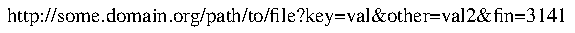
\includegraphics[trim = 30 30 30 30,width=1cm]{images/url/url.pdf}};
			\node (feature) at (4,0) {$x=\left\{\begin{array}{c}(x_{1,1},\ldots,x_{1,d}) \\ (x_{2,1},\ldots,x_{2,d}) \\ \vdots \\(x_{b,1},\ldots,x_{b,d}) \end{array} \right\}$};
				\node (classifier) at (9,0) {$f(x)=\begin{cases} +1 \\ -1\end{cases}$};
					\draw [->] (apple.east) -- (feature.west) node [pos=0.5,above] {extract};
					\draw [->] (apple.east) -- (feature.west) node [pos=0.5,below] {features};
					\draw [->] (feature.east) -- (classifier.west) node [pos=0.5,above] {send to};
					\draw [->] (feature.east) -- (classifier.west) node [pos=0.5,below] {classifier};
		\end{tikzpicture}
	\end{center}
\end{frame}


\begin{frame}[c]\frametitle{Embedding methods for multi-instance learning}
	\begin{center}
		\begin{tikzpicture}
			\node (apple) at (0,0) {$\left\{\begin{array}{c}(x_{1,1},\ldots,x_{1,d}) \\ (x_{2,1},\ldots,x_{2,d}) \\ \vdots \\(x_{b,1},\ldots,x_{b,d}) \end{array} \right\}$};
				\node (feature) at (5,0) {$\bar{x}\in\mathbb{R}^m$};
				\node (classifier) at (9,0) {$f(\bar{x})=\begin{cases} +1 \\ -1\end{cases}$};
					\draw [->] (apple.east) -- (feature.west) node [pos=0.5,above] {$\phi(b)$ embeds} node [pos=0.5,below] {bag to};
					\draw [->] (feature.east) -- (classifier.west) node [pos=0.5,above] {send to};
					\draw [->] (feature.east) -- (classifier.west) node [pos=0.5,below] {classifier};
		\end{tikzpicture}
	\end{center}
\end{frame}

\begin{frame}{MIL5}
	\begin{tikzpicture}
		\tikzstyle{vector}=[inner sep=1pt]
		\tikzstyle{function}=[rectangle,rounded corners=7pt,draw,minimum width=1cm,inner sep=3pt]

		\foreach \y/\i in {2/1,1/2,0/3,-2/l}
		  \node[vector] (x\i) at (-2,\y)  {$x_{\i}\in\mathbb{R}^d$};
		  \node at (-2,-1)  {$\vdots$};

		  \foreach \y/\i in {2/1,1/2,0/3,-2/l}
		    \node[function] (h\i) at (0,\y)  {$h(x_{\i},\theta_h)$};


			\foreach \y/\i in {2/1,1/2,0/3,-2/l}
			  \node[vector] (xtilde\i) at (2,\y)  {$\tilde{x}_{\i}\in\mathbb{R}^u$};
			  \node at (2,-1)  {$\vdots$};
			  \foreach \i in {1,2,3,l}
			    \draw[->] ($(x\i.east)+(+0,0)$) -- ($(h\i.west)+(0,0)$) ;
				\foreach \i in {1,2,3,l}
				  \draw[->] ($(h\i.east)+(+0,0)$) -- ($(xtilde\i.west)+(-0,0)$) ;

				  \node[function] (g) at (5,0) {$g\left(\lbrace\tilde{x}_i\rbrace_{i=1}^l,\theta_g\right)$}; 
				  \foreach \i in {1,2,3,l}
				    \draw[->] ($(xtilde\i.east)+(+0,0)$) -- ($(g.west)+(-0,0)$) ;
					\node[vector] (xbar) at (7.5,0)  {$\bar{x}\in\mathbb{R}^u$};
					\draw[->] ($(g.east)+(+0,0)$) -- ($(xbar.west)+(-0,0)$) ;

					% \node at (1,-1)  {$\vdots$};


					\node[function] (f) at (9,0) {$f\left(\bar{x},\theta_f\right)$}; 
					\draw[->] ($(xbar.east)+(+0,0)$) -- ($(f.west)+(-0,0)$) ;

					\node[] at (5,-5) {$g\left(\lbrace\tilde{x}_i\rbrace_{i=1}^l\right)=\frac{1}{l}\sum_{i=1}^l \tilde{x}_i$};
					\node[] at (0,-5) {$h(x,\theta_h)=\max\lbrace 0,x^{\mathrm{T}}\theta_h\rbrace$};
					\node[] at (9,-5) {$f(\bar{x},\theta_f)=\bar{x}^{\mathrm{T}}\theta_f$};
					\draw [thick,decoration={brace,mirror,raise=0.5cm},decorate] (xl.west) -- (xtildel.east) node [pos=0.5,anchor=north,yshift=-0.55cm] {One vector per instance (connection)}; 

					\draw [thick,decoration={brace,mirror,raise=0.5cm},decorate] (g.east) -- (f.east) node [pos=0.5,anchor=north,yshift=-0.55cm] {One vector per sample}; 
					% \begin{scope}[opacity=0]
					% \end{scope}
	\end{tikzpicture}
\end{frame}

\end{document}
